\section{Test: Linear model} \label{sec:test_lin}
The purpose of this chapter is to show and discuss some of the performance results of the LQI controller derived in \cref{sec:ctrl-design} on the linear model derived in \cref{sec:linear_model}. Only a few of the results are shown here and the rest can be found in the appendix in \cref{sec:app_test_lin} which also contains a description of the test setup. The controller is benchmarked against the original FLC controller with regards to both rotor speed control and fore-aft movement dampening capability. Simulations on the linear model were run initially to confirm the correctness of the linear model and the controller performance with initial LQI weight guesses. Prior to this test the LQI controller has been tuned such that a satisfactory performance was achieved in VTS.

It is expected that the LQI controller will perform much better in damping the fore-aft movement than the original FLC PI controller with no FATD. Results are shown for both frequency and time domain.


\subsection{Frequency domain}
The frequency domain analysis shows that the LQI controller performs better in dampening the effect of the disturbance on both the fore-aft movement and the rotor speed. The plot in \cref{fig:script_vfreeTovy} has been included here and it shows the frequency response from the free wind disturbance $ v_{free} $ to the fore-aft tower top velocity $ v_y $. Both the FLC PI system and LQI system are plotted for comparison. It is observed that the LQI controller yields much greater dampening of the eigenfrequency than the FLC PI controller. This is of course expected because the FLC controller is tuned for fixed-bottom turbine control.
\begin{figure}[ht]
	\centering
	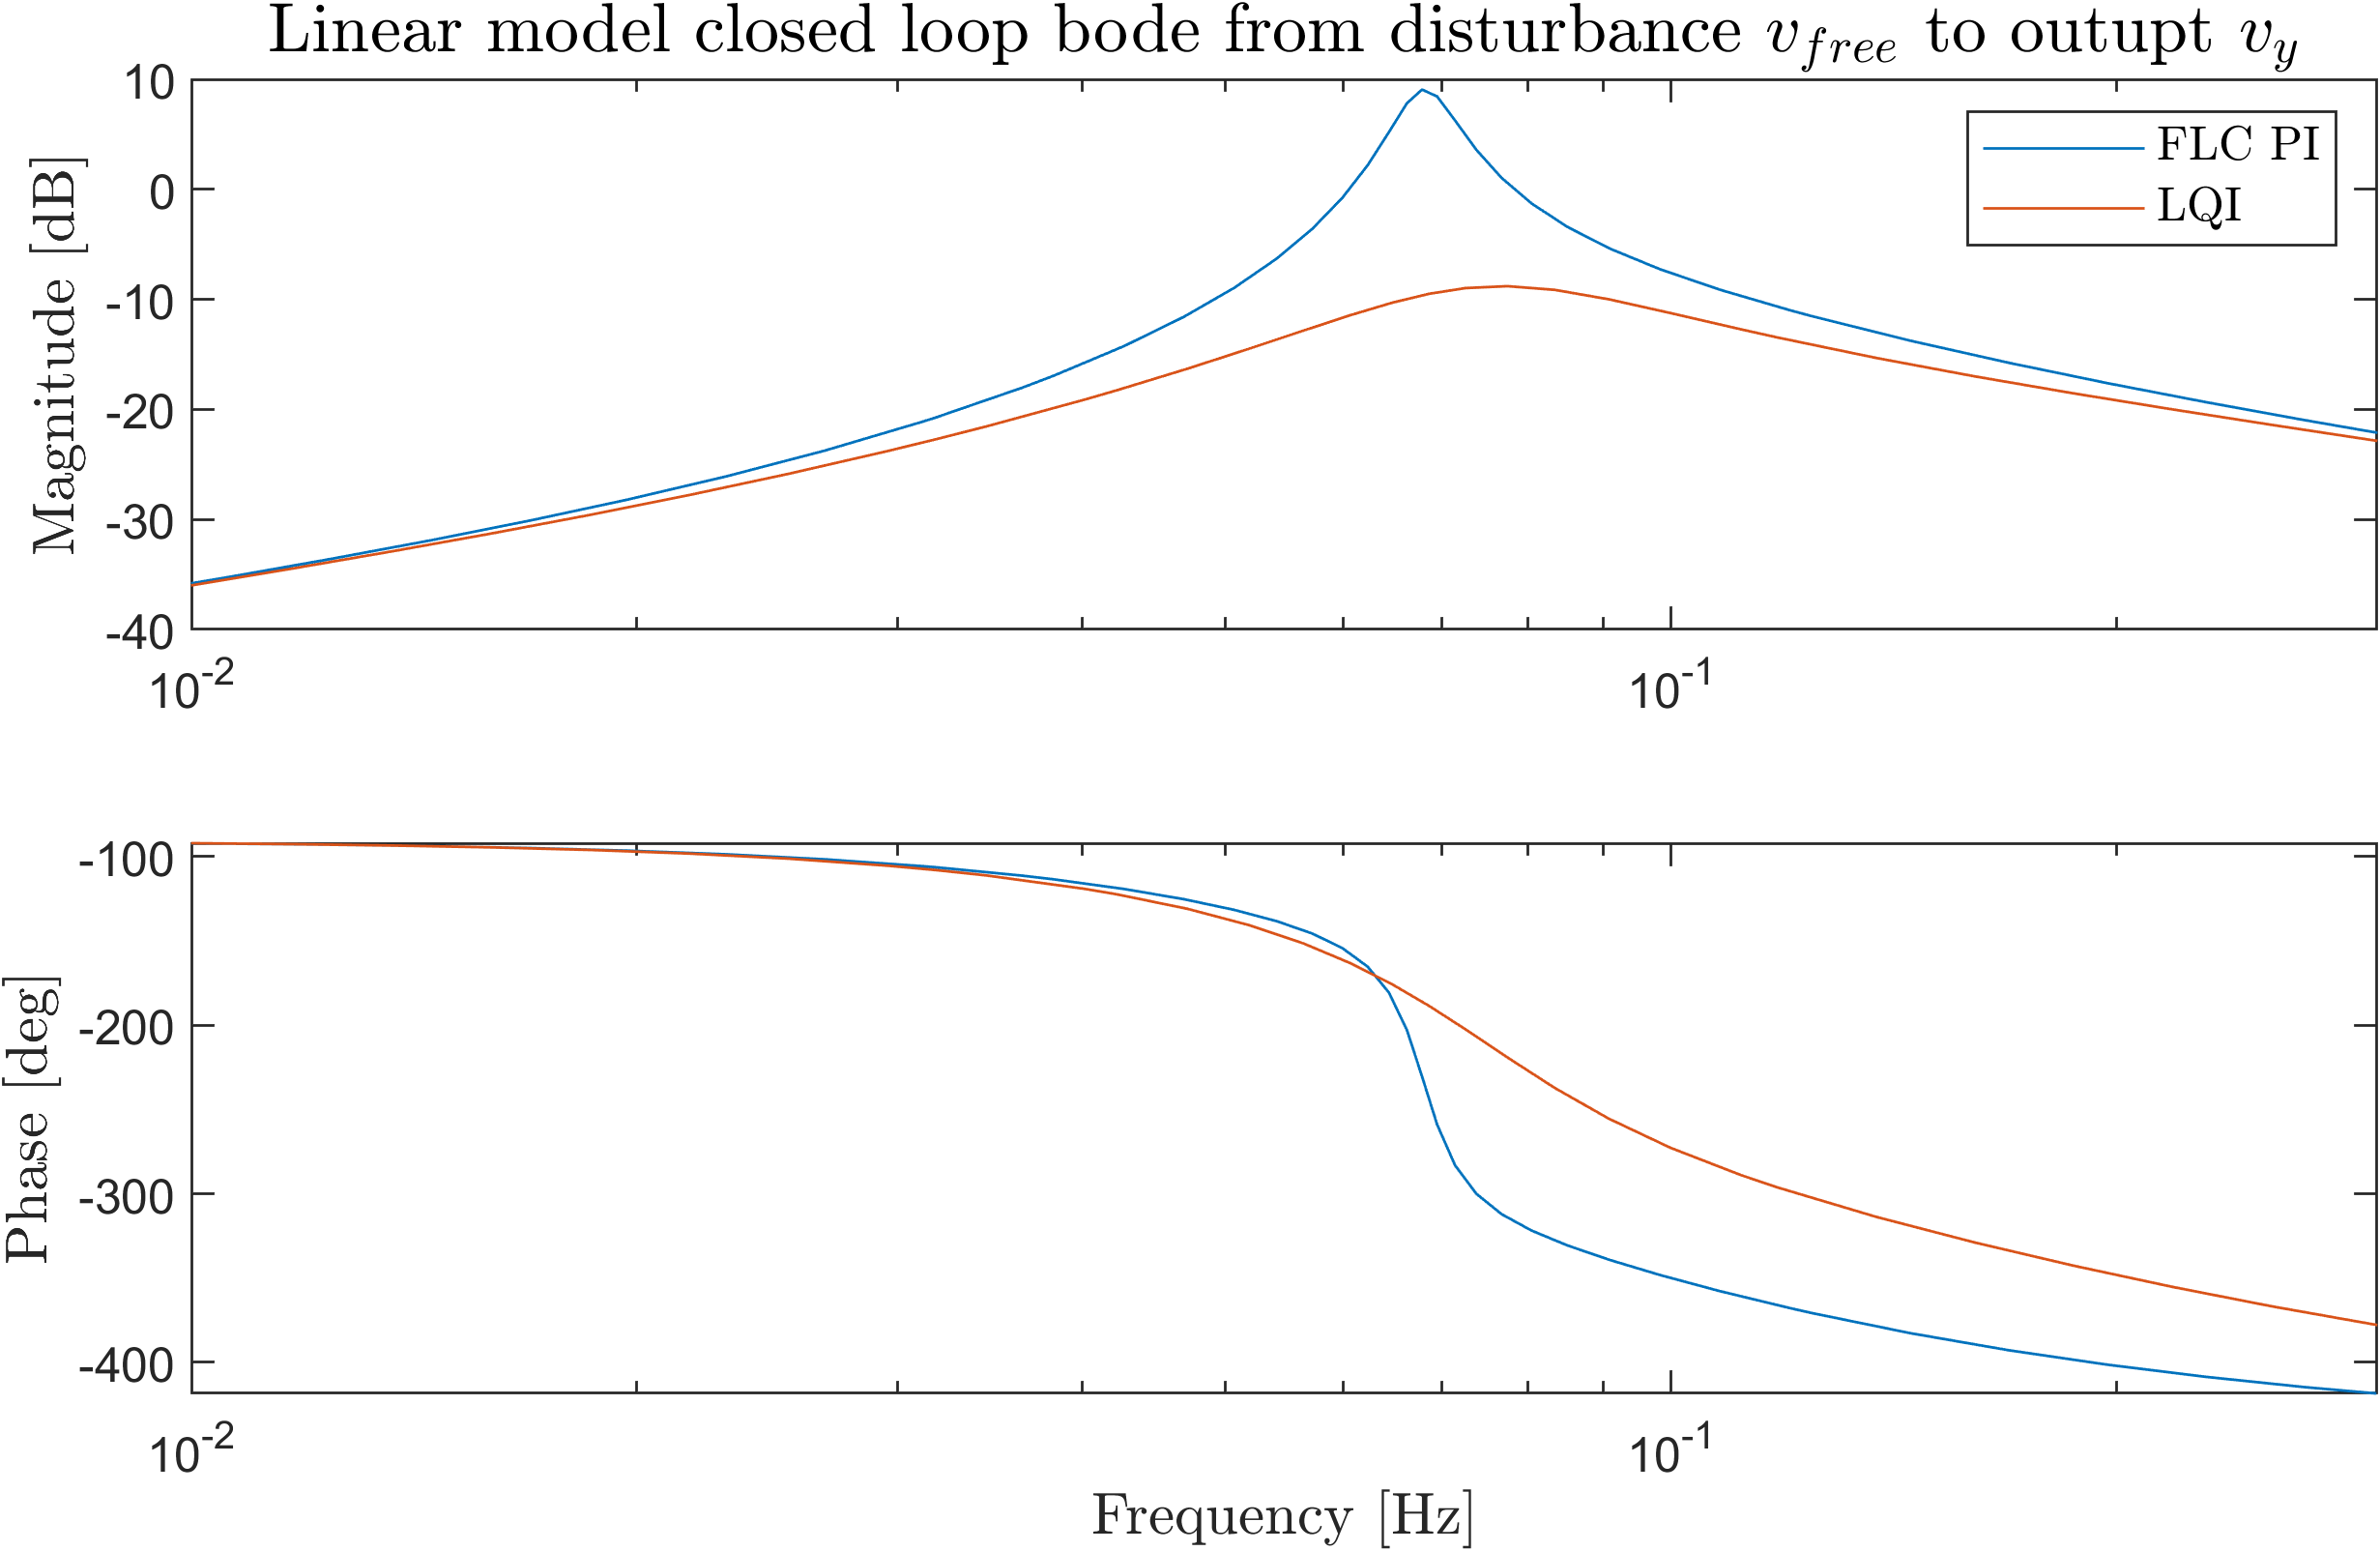
\includegraphics[width=0.7\linewidth]{Graphics/TestResults/linearModPerf/script_vfreeTovy.png}
	\caption{Frequency response from the free wind as observed by the rotor ($ v_{free} $) to the fore-aft velocity ($ v_y $) of the linear model with a comparison between the original FLC PI controller and the LQI controller. Much better disturbance dampening is gained from the LQI controller.}
	\label{fig:script_vfreeTovy}
\end{figure}


\clearpage
\subsection{Time domain}
Time domain simulations were executed with Matlab Simulink for 1000 seconds and the results plotted with Matlab. In \cref{fig:sim_11_W_py_vy_comp} the rotor speed, fore-aft (surge direction) position and velocity is plotted. Both the FLC PI and LQI controlled systems are plotted for comparison. Both rotor speed tracking and fore-aft motion damping performance is vastly superior for the LQI controller. The poor rotor speed tracking performance of the FLC controller is expected because of its lack of consideration for the fore-aft motion. The pitch actuation activity from the LQI controller furthermore does not exceed alarming values.
\begin{figure}[ht]
	\centering
	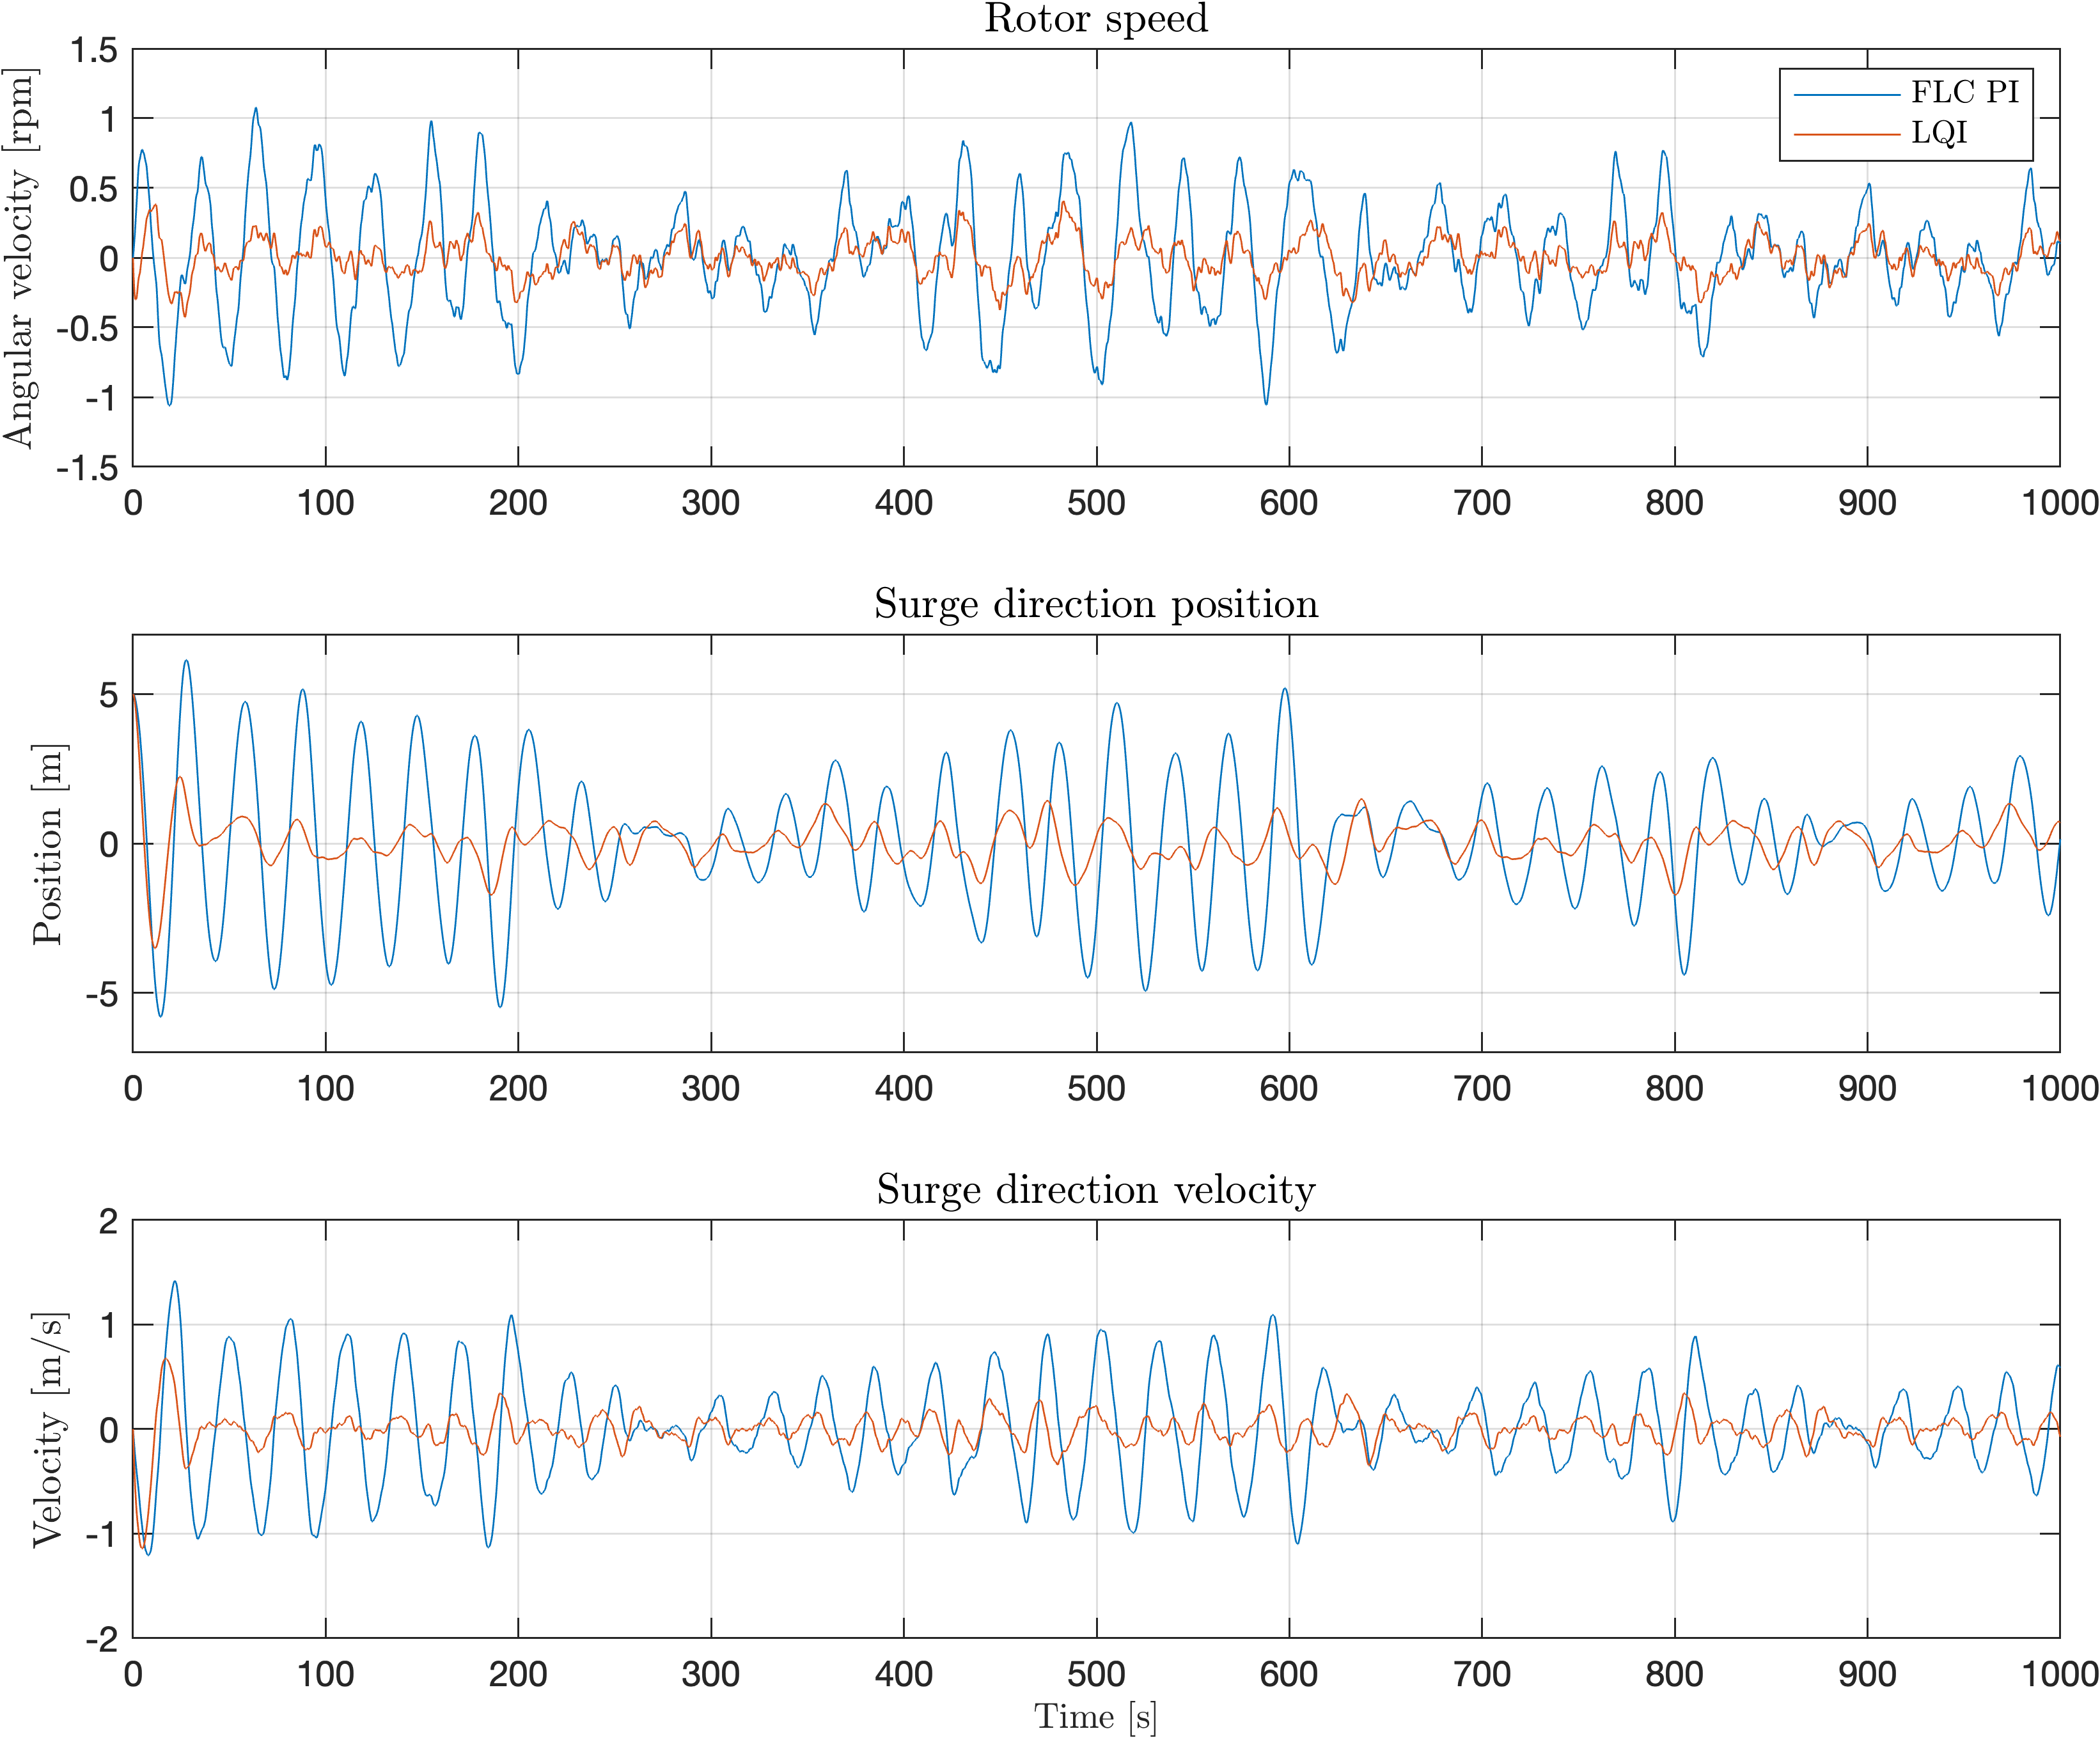
\includegraphics[width=0.7\linewidth]{Graphics/TestResults/linearModPerf/sim_11_W_py_vy_comp.png}
	\caption{Simulink simulation results. The 5 m deviation initialization of the tower top position is visible from the \textit{fore-aft position} at 0 s.}
	\label{fig:sim_11_W_py_vy_comp}
\end{figure}